% begin module polar-curve-ex6
\begin{frame}[t]
\begin{example} %[Example 6, p. 678]
\begin{enumerate}
\item<1-| alert@2-21> Sketch the curve with polar equation \alertNoH{ 26}{$r = 2\cos \theta$}.
\item<1-| alert@22-> Find a Cartesian equation for this curve.
\end{enumerate}
\begin{columns}[c]
\column{.5\textwidth}
\psset{xunit=1.75cm, yunit=1.75cm}
\begin{pspicture}(-0.6, -1.5)(2.5,1.5)

\tiny
\fcAxesStandard{-0.52}{-1.4}{2.4}{1.4}

\uncover<21->{
%Calculator input: plotCurve{}(2 \cos^{2}{}t, 2 \cos{}t \sin{}t, 0, 2 \pi)
\parametricplot[linecolor=\fcColorGraph, plotpoints=200]{0}{6.28319}{t 57.29578 mul cos 2.0000000 exp 2.0000000 mul t 57.29578 mul sin t 57.29578 mul cos mul 2.0000000 mul }
}
\uncover<4->{
\fcFullDot{2}{0}
\rput[bl](2.05,0.05){$(2,0)$}
}
\uncover<6->{
\fcFullDot{1.500000}{0.866025}
\rput[bl](1.55,0.9){$\left(\sqrt{3}, \frac{\pi}{6}\right)$}
}

\uncover<8->{
\fcFullDot{1}{1}
\rput[bl](1.05,1.05){$\left(\sqrt{2}, \frac{\pi}{4}\right)$}
}
\uncover<10->{
\fcFullDot{0.5}{0.866025}
\rput[br](0.45,0.86){$\left(1, \frac{\pi}{3}\right)$}
}
\uncover<12->{
\fcFullDot{0}{0}
\rput[tr](-0.05,-0.05){$\left(0,\frac{\pi}{2}\right)$}
}
\uncover<14->{
\fcFullDot{0.5}{ -0.866025}
\rput[t](0.5,-0.88){$\left(-1, \frac{2\pi}{3}\right)$}
}
\uncover<16->{
\fcFullDot{1}{-1}
\rput[t](1,-1.05){$\left(-\sqrt{2},\frac{3\pi}{4}\right)$}
}
\uncover<18->{
\fcFullDot{1.5}{-0.866025}
\rput[lt](1.5,-0.9){$\left(-\sqrt{3},\frac{5\pi}{6}\right)$}
}
\uncover<4-5>{
\psline[linecolor=blue](0,0)(2,0)
}
\uncover<6-7>{
\parametricplot[arrows=->, linecolor=\fcColorGraph, plotpoints=200] {0}{0.523598776 }{t 57.29578 mul cos 0.3 mul t 57.29578 mul sin 0.3 mul }
\psline[linecolor=blue](0,0)(1.5,0.866025)
}
\uncover<8-9>{
\parametricplot[arrows=->, linecolor=\fcColorGraph, plotpoints=200] {0}{0.785398163}{t 57.29578 mul cos 0.3 mul t 57.29578 mul sin 0.3 mul }
\psline[linecolor=blue](0,0)(1,1)
}
\uncover<10-11>{
\parametricplot[arrows=->, linecolor=\fcColorGraph, plotpoints=200] {0}{1.047197551}{t 57.29578 mul cos 0.3 mul t 57.29578 mul sin 0.3 mul }
\psline[linecolor=blue](0,0)(0.5,0.866025)
}
\uncover<12-13>{
\parametricplot[arrows=->, linecolor=\fcColorGraph, plotpoints=200] {0}{1.570796327}{t 57.29578 mul cos 0.3 mul t 57.29578 mul sin 0.3 mul }
}
\uncover<14-15>{
\parametricplot[arrows=->, linecolor=\fcColorGraph, plotpoints=200] {0}{2.094395102}{t 57.29578 mul cos 0.3 mul t 57.29578 mul sin 0.3 mul }
\psline[linecolor=blue](0,0)(0.5, -0.866025)
\psline[linecolor=blue, linestyle=dashed](0,0)(-0.500000, 0.866025)
}
\uncover<16-17>{
\parametricplot[arrows=->, linecolor=\fcColorGraph, plotpoints=200] {0}{2.35619449}{t 57.29578 mul cos 0.3 mul t 57.29578 mul sin 0.3 mul }
\psline[linecolor=blue, linestyle=dashed](0,0)(-0.5, 0.5)
\psline[linecolor=blue](0,0)(1, -1)
}
\uncover<18-19>{
\parametricplot[arrows=->, linecolor=\fcColorGraph, plotpoints=200] {0}{2.617993878}{t 57.29578 mul cos 0.3 mul t 57.29578 mul sin 0.3 mul }
\psline[linecolor=blue, linestyle=dashed](0,0)(-0.500000, 0.288675)
\psline[linecolor=blue](0,0)(1.500000, -0.866025)
}
\uncover<20>{
\parametricplot[arrows=->, linecolor=\fcColorGraph, plotpoints=200] {0}{3.141592654}{t 57.29578 mul cos 0.3 mul t 57.29578 mul sin 0.3 mul }
\psline[linecolor=blue, linestyle=dashed](0,0)(-0.5,0)
\psline[linecolor=blue](0,0)(2,0)
}
\end{pspicture}
\vspace{1cm}
%\ \only<handout:0| -3>{%
%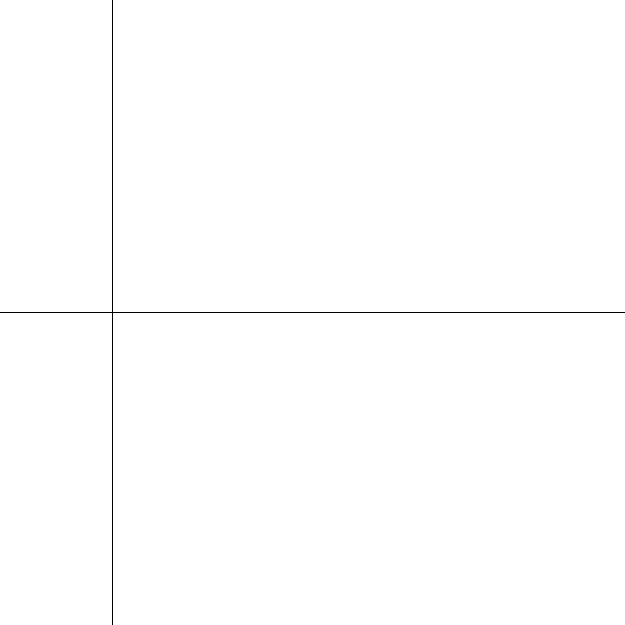
\includegraphics[height=6cm]{polar-curves/pictures/11-03-ex6z.pdf}%
%}%
%\only<handout:0| 4-5>{%
%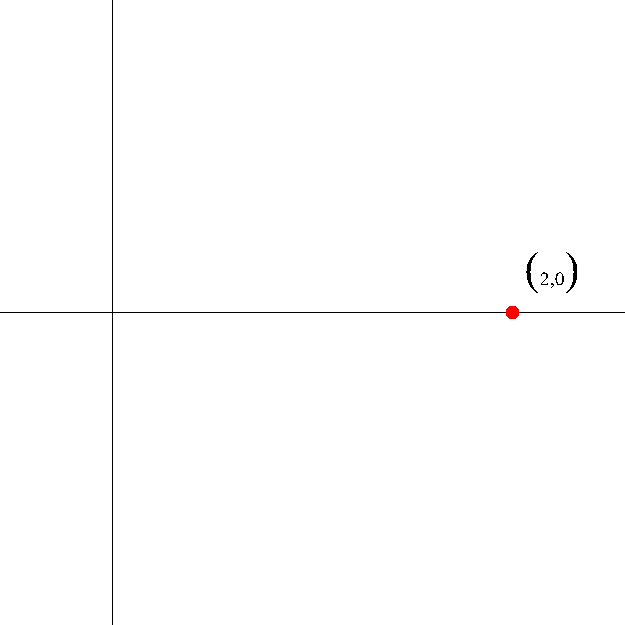
\includegraphics[height=6cm]{polar-curves/pictures/11-03-ex6a.pdf}%
%}%
%\only<handout:0| 6-7>{%
%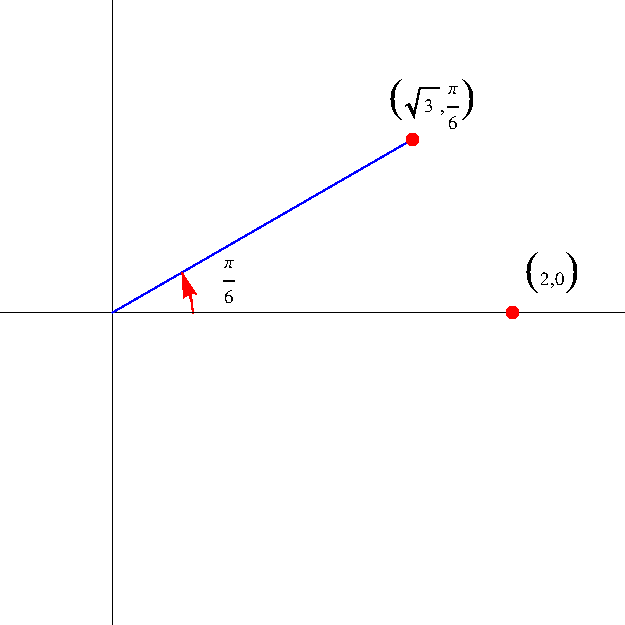
\includegraphics[height=6cm]{polar-curves/pictures/11-03-ex6b.pdf}%
%}%
%\only<handout:0| 8-9>{%
%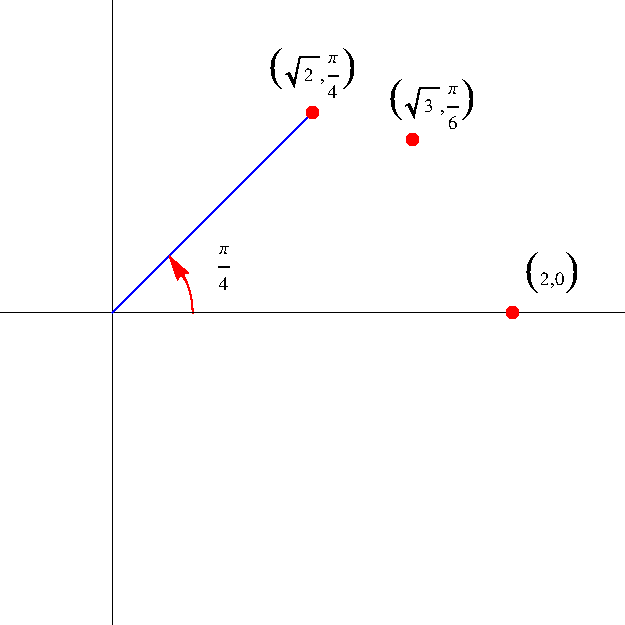
\includegraphics[height=6cm]{polar-curves/pictures/11-03-ex6c.pdf}%
%}%
%\only<handout:0| 10-11>{%
%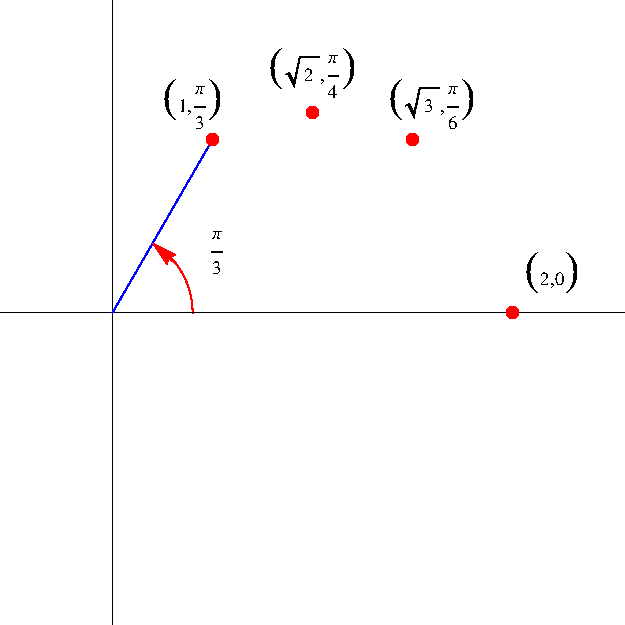
\includegraphics[height=6cm]{polar-curves/pictures/11-03-ex6d.pdf}%
%}%
%\only<handout:0| 12-13>{%
%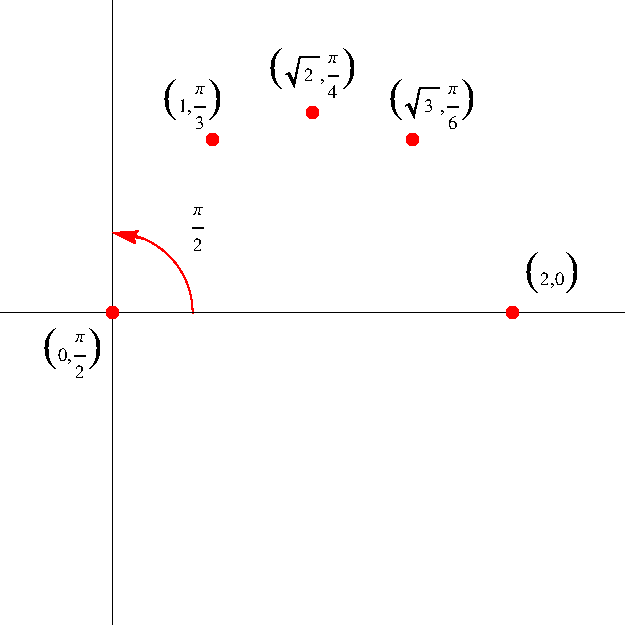
\includegraphics[height=6cm]{polar-curves/pictures/11-03-ex6e.pdf}%
%}%
%\only<handout:0| 14-15>{%
%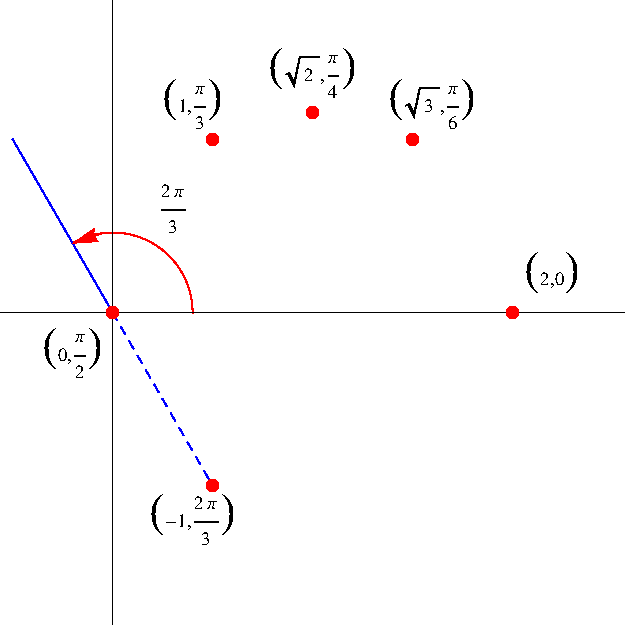
\includegraphics[height=6cm]{polar-curves/pictures/11-03-ex6f.pdf}%
%}%
%\only<handout:0| 16-17>{%
%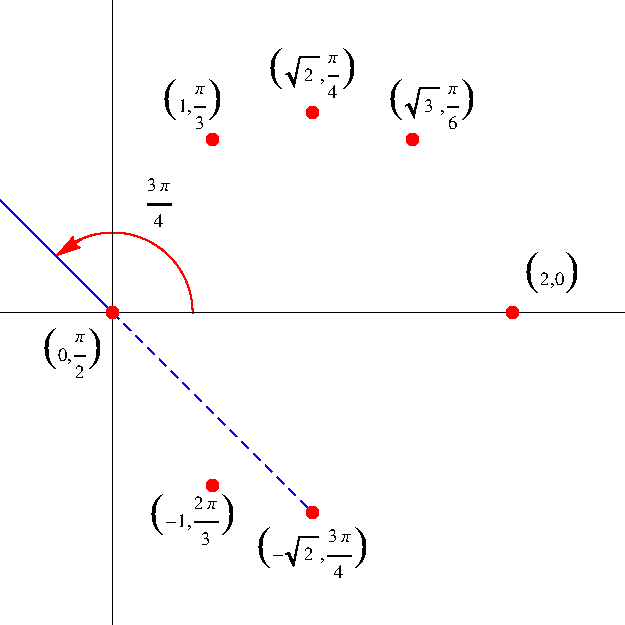
\includegraphics[height=6cm]{polar-curves/pictures/11-03-ex6g.pdf}%
%}%
%\only<handout:0| 18-19>{%
%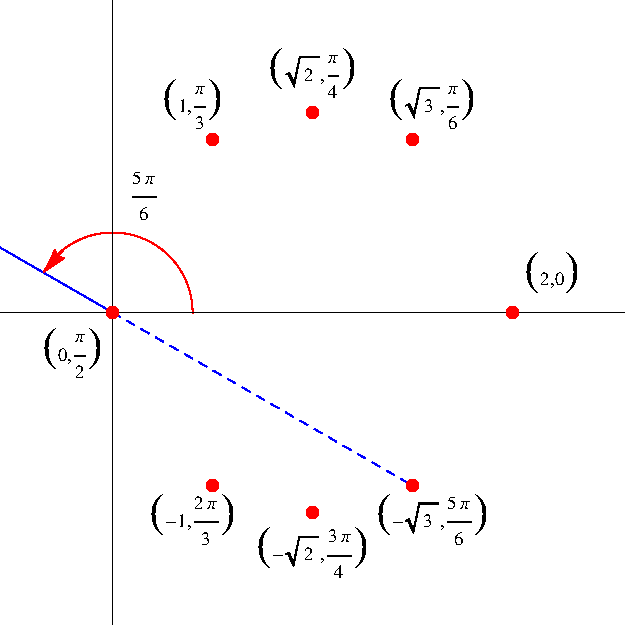
\includegraphics[height=6cm]{polar-curves/pictures/11-03-ex6h.pdf}%
%}%
%\only<handout:0| 20>{%
%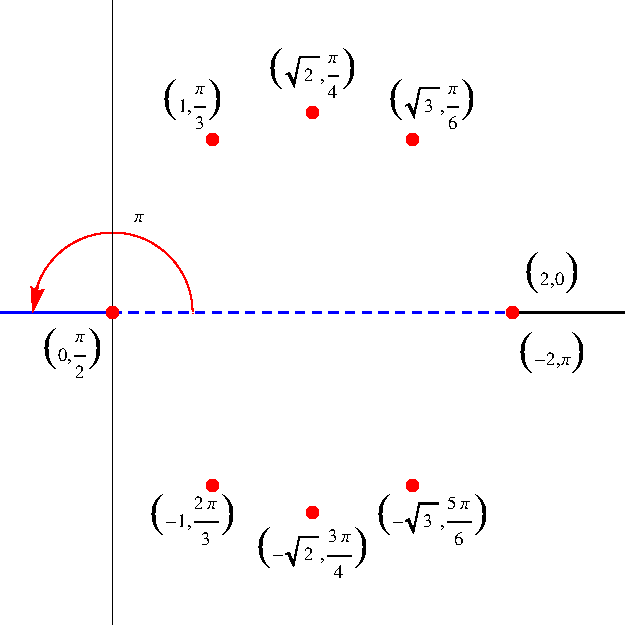
\includegraphics[height=6cm]{polar-curves/pictures/11-03-ex6i.pdf}%
%}%
%\only<21->{%
%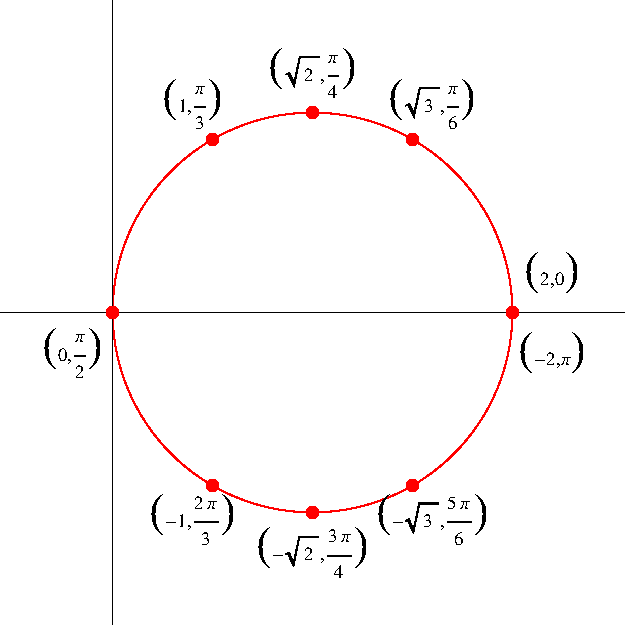
\includegraphics[height=6cm]{polar-curves/pictures/11-03-ex6j.pdf}%
%}%
\column{.5\textwidth}
\only<handout:1| -21>{\uncover<2->{%
\[
\begin{array}{|@{\ }l@{\ }|r@{\ }|}
\hline
\theta & r \\
\hline
\alertNoH{ 3-4}{%
0%
}&%
\uncover<4->{\alertNoH{ 4}{%%
2%
}}\\%%
\alertNoH{ 5-6}{%
\pi /6%
}&%
\uncover<6->{\alertNoH{ 6}{%%
\sqrt{3}%
}}\\%%
\alertNoH{ 7-8}{%
\pi /4%
}&%
\uncover<8->{\alertNoH{ 8}{%%
\sqrt{2}%
}}\\%%
\alertNoH{ 9-10}{%
\pi /3%
}&%
\uncover<10->{\alertNoH{ 10}{%%
1%
}}\\%%
\alertNoH{ 11-12}{%
\pi /2%
}&%
\uncover<12->{\alertNoH{ 12}{%%
0%
}}\\%%
\alertNoH{ 13-14}{%
2\pi /3%
}&%
\uncover<14->{\alertNoH{ 14}{%%
-1%
}}\\%%
\alertNoH{ 15-16}{%
3\pi /4%
}&%
\uncover<16->{\alertNoH{ 16}{%%
-\sqrt{2}%
}}\\%%
\alertNoH{ 17-18}{%
5\pi /6%
}&%
\uncover<18->{\alertNoH{ 18}{%%
-\sqrt{3}%
}}\\%%
\alertNoH{ 19-20}{%
\pi%
}&%
\uncover<20->{\alertNoH{ 20}{%%
-2%
}}\\%%
\hline
\end{array}
\]
}}%
\only<handout:2| 22->{%
\begin{itemize}
\item<22-| alert@22-23>  $x = $ \uncover<23->{$r\cos \theta$.}
\item<24-| alert@24-25>  $\cos \theta = $ \uncover<25->{$x/r$.}
\item<26-| alert@26-27>  $r = 2\cos \theta = $ \uncover<27->{$\alertNoH{ 28}{2x}/r$.}
\item<28-| alert@28-30>  $2x = $ \uncover<29->{$r^2 = $ \uncover<30->{$x^2+y^2$.}}
\item<31->  $x^2 + y^2 - 2x = 0$.
\item<32->  Complete the square:
\end{itemize}
\begin{eqnarray*}
\uncover<32->{%
(x^2 - 2x \uncover<33->{\alertNoH{ 33}{+ 1}}) + y^2%
}%
& \uncover<32->{ = } &%
\uncover<32->{%
0 \uncover<33->{\alertNoH{ 33}{+ 1}}%
}\\%
\uncover<34->{%
(x-1)^2 + y^2%
}%
& \uncover<34->{ = } &%
\uncover<34->{%
1%
}%
\end{eqnarray*}
}%
\end{columns}
\end{example}
\end{frame}
% end module polar-curve-ex6
